\documentclass{scrartcl}
\usepackage{lscape}
\usepackage{tikz}

\begin{document}
%\begin{landscape}
\centering
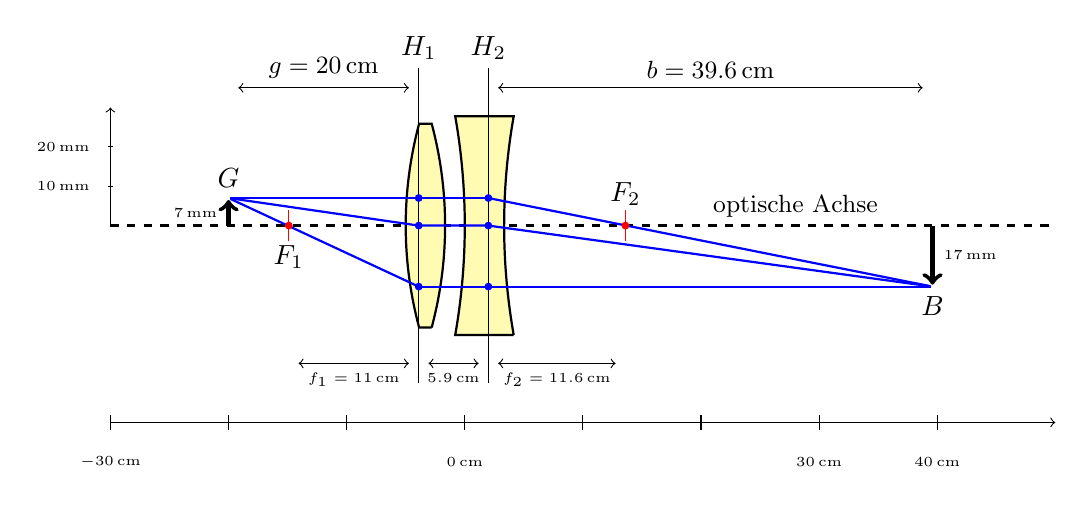
\begin{tikzpicture}[scale=0.5]%, inner sep=0]
\def\sx{0.3}

% Optische Achse
\draw[dashed, thick] (-30*\sx,0) -- (50*\sx,0);
% Koordinaten Nullpunkt
\draw (0,-0.2) -- (0,0.2);

% Konkave Linse
\def\xconv{0.5} % x-Koordinate
\draw[thick, fill=yellow!30] 
     ([shift=(190:16cm)]16.5+\xconv,0) arc (190:170:16cm)
     -- ([shift=(10:16cm)] -16.5+\xconv,0)
     arc (10:-10:16cm) 
     -- ([shift=(190:16cm)]16.5+\xconv,0);

% Konvexe Linse
\def\xconx{-1.5} % x-Koordinate
\draw[thick, fill=yellow!30] ([shift=(-15:10cm)]-9+\xconx,0) arc (-15:15:10cm)
 --([shift=(165:10cm)]10+\xconx,0) arc (165:195:10cm)
 --([shift=(-15:10cm)]-9+\xconx,0);

% Gegenstand (Pfeil)
\def\Gx{-20.0*\sx}
\def\Gy{0.7}
\node [inner sep=0] (G) at (\Gx,\Gy) {};
\draw[->, ultra thick, left] (\Gx,0) to node {\tiny $7\,$mm} (G);%
\node (labG) at (\Gx,\Gy+0.5) {$G$};
% Bild (arrow)
\def\Bx{39.6*\sx}
\def\By{-1.55}
\node[inner sep=0] (B) at (\Bx,\By) {};
\draw[->, ultra thick, right] (\Bx,0) to node {\tiny $17\,$mm}  (B);
\node (labB) at (\Bx,\By-0.5) {$B$};

% Hauptebenen
\def\Hx{-3.9*\sx}
\def\Hxii{2.0*\sx}
\draw (\Hx,-4) -- (\Hx,4); % H1
\node (labH1) at (\Hx,4.5) {$H_1$};
\draw (\Hxii,-4) -- (\Hxii,4); % H2
\node (labH2) at (\Hxii,4.5) {$H_2$};

% Strahlen
% FokusG
\fill[blue] (\Hx,\By) circle [radius=0.1];
\fill[blue] (\Hxii,\By) circle [radius=0.1];
\fill[blue] (\Hx,0) circle [radius=0.1];
\fill[blue] (\Hx,\Gy) circle [radius=0.1];
\fill[blue] (\Hxii,\Gy) circle [radius=0.1];
\fill[blue] (\Hxii,0) circle [radius=0.1];
\draw[thick, color=blue] (G) -- (\Hx,\By);
\draw[thick, color=blue] (B) -- (\Hx,\By);
% FokusB
\draw[thick, color=blue] (G) -- (\Hxii,\Gy);
\draw[thick, color=blue] (B) -- (\Hxii,\Gy);
%Central
\draw[thick, color=blue] (G) -- (\Hx,0) -- (\Hxii,0)  -- (B);
               
% Label
%Fokus Punkte
\def\fxi{-11*\sx+\Hx}
\def\fxii{11.6*\sx+\Hxii}
\draw[red] (\fxi,-0.4) -- (\fxi,0.4);
\draw[red] (\fxii,-0.4) -- (\fxii,0.4);
\fill[red] (\fxi,0) circle [radius=0.1];
\fill[red] (\fxii,0) circle [radius=0.1];
\node (F1) at (\fxi,-0.8) {$F_1$};
\node (F2) at (\fxii,0.8) {$F_2$};
% Distanzen
\node (f1) at (\fxi,-3.5) {} ;
\node (h1) at (\Hx,-3.5) {} ;
\node (f2) at (\fxii,-3.5) {} ;
\node (h2) at (\Hxii,-3.5) {} ;
\draw[<->, below] (f1) to node {\tiny $f_1=11\,$cm} (h1) ;
\draw[<->, below] (f2) to node {\tiny $f_2=11.6\,$cm} (h2) ;
\draw[<->, below]%, inner sep=10] 
(h1) to node {\tiny $5.9\,$cm} (h2);

\node (g) at (\Gx,3.5) {} ;
\node (gh1) at (\Hx,3.5) {} ;
\node (b) at (\Bx,3.5) {} ;
\node (bh2) at (\Hxii,3.5) {} ;
\draw[<->, above] (g) to node {\small $g=20\,$cm} (gh1) ;
\draw[<->, above] (b) to node {\small $b=39.6\,$cm} (bh2) ;

% Koordinaten Nullpunkt
% x-Achse
\def\cy{-5}
\draw[->] (-30*\sx,\cy) -- (50*\sx,\cy);
\draw (0,-0.2+\cy) -- (0,0.2+\cy);
\draw (10*\sx,-0.2+\cy) -- (10*\sx,0.2+\cy);
\draw (-10*\sx,-0.2+\cy) -- (-10*\sx,0.2+\cy);
\draw (20*\sx,-0.2+\cy) -- (20*\sx,0.2+\cy);
\draw (-20*\sx,-0.2+\cy) -- (-20*\sx,0.2+\cy);
\draw (30*\sx,-0.2+\cy) -- (30*\sx,0.2+\cy);
\draw (-30*\sx,-0.2+\cy) -- (-30*\sx,0.2+\cy);
\node (m30) at (-30*\sx,-1+\cy) {\tiny $-30\,\mathrm{cm}$};
\node (p30) at (30*\sx,-1+\cy) {\tiny $30\,\mathrm{cm}$};
\node (zero) at (0*\sx,-1+\cy) {\tiny $0\,\mathrm{cm}$};
\draw (40*\sx,-0.2+\cy) -- (40*\sx,0.2+\cy);
\node (p40) at (40*\sx,-1+\cy) {\tiny $40\,\mathrm{cm}$};

\node (Achse) at (28*\sx,0.5) {\small optische Achse};

% y-Achse
\draw[->] (-30*\sx,0) -- (-30*\sx,3);
\draw (-30.2*\sx,1) -- (-29.8*\sx,1);
\node (y10) at (-34*\sx,1) {\tiny $10\,\mathrm{mm}$};
\draw (-30.2*\sx,2) -- (-29.8*\sx,2);
\node (y20) at (-34*\sx,2) {\tiny $20\,\mathrm{mm}$};

% Gebogener Pfeil
%\draw[->, dashed] (9.5,18) .. controls (4,18) .. (3,11.65);
\end{tikzpicture}
%\end{landscape}
\end{document}